%Dimensionality reduction techniques should be on the agenda for anyone interested in more visualizing complex data. 

Multi-dimensional scaling is a kind of dimensionality reduction, allowing one to translate a set of items and their predetermined pairwise distances into an arrangement of points in Cartesian space, typically in two dimensions. This is not a trivial task. Consider the meme below, which references social distancing guidance from the coronavirus pandemic. We have four individuals, forming six possible pairs, and any two individuals must maintain a six-foot distance. The graphic shows impossible right triangles that violate the Pythagorean Theorem when the distances are all exactly six feet. Indeed, there is no way to arrange four individuals in two-dimensional space so that they are all exactly six feet apart. This highlights one difficulty in multi-dimensional scaling---we must accept some error in our output. 

\begin{center}
    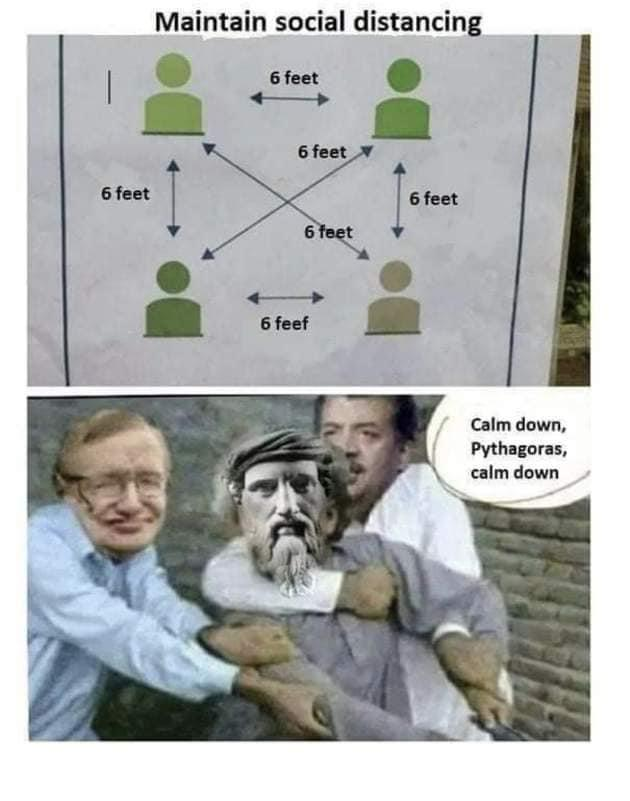
\includegraphics[width = 0.8\textwidth]{images/calmdownpythag.jpg}
\end{center}

\vspace{-2cm}

The following diagram helps show why no alternative arrangement could be perfect. Each point $a,b,c$ is in the middle of a circle of six-foot radius. For $b$ to be six feet away from $a$, $b$ must lie on the circle centered at $a$. Similarly, for $b$ to be six feet away from $c$, $b$ must also lie on the circle centered at $c$. For three points, this arrangement is possible. But if we introduce $d$, $d$ must lie on all three of the circles centered at $a$, $b$, and $c$. But there is no point where all three circles intersect.\footnote{The code is (link TK).}

\begin{center}
    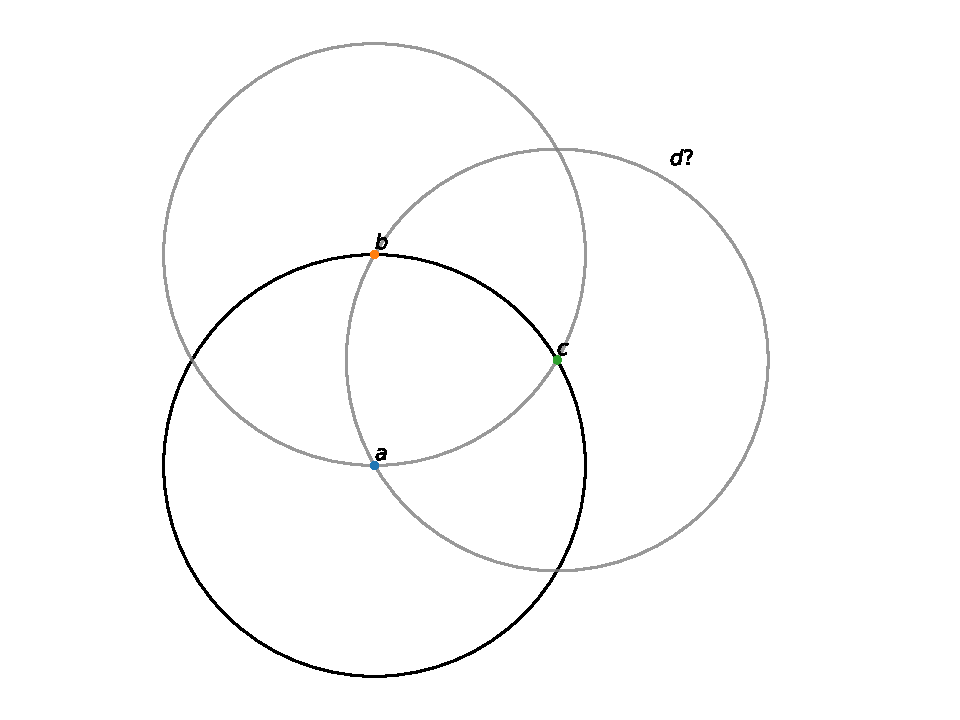
\includegraphics[width = 0.96\textwidth]{figures/specialplots/mds-circles.pdf}
\end{center}

%\pyfile{mds-circles.py}

Suppose we have four points, with unit pairwise distances for any two distinct points. Applying multi-dimensional scaling creates what is roughly a square.

\begin{center}
    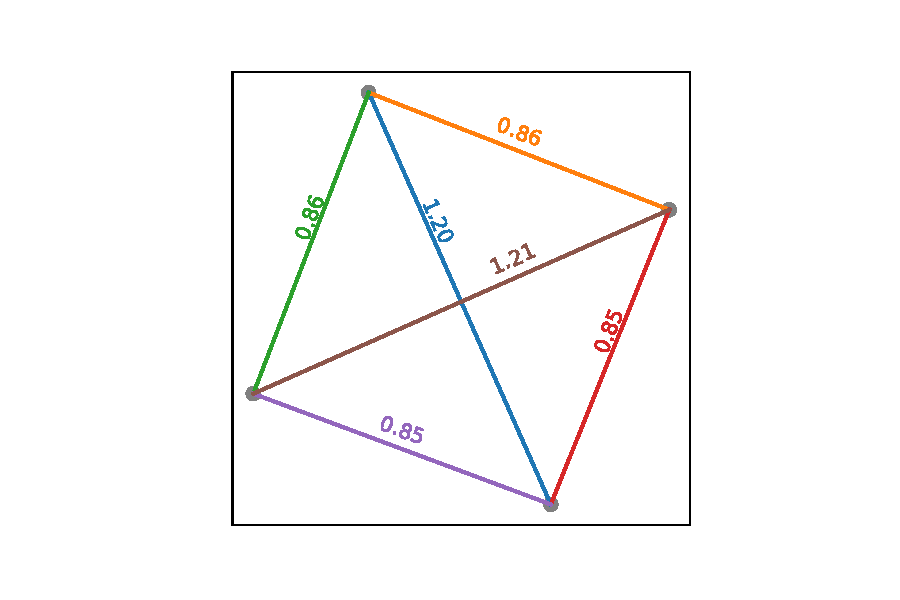
\includegraphics[width = 0.96\textwidth]{Images/MDS_social.pdf}
\end{center}

TKTK